\documentclass{article}
\usepackage{amsthm,amsmath,amsfonts,lipsum}
\usepackage[T1]{fontenc}
\usepackage{beramono}
\usepackage{listings}
\usepackage{fontawesome5}
\usepackage{adjustbox}
\usepackage{mathabx}
\usepackage{thmtools}
\usepackage{import}
\usepackage{graphicx}
\usepackage{setspace}
\usepackage{geometry}
\usepackage{physics}
\usepackage{float}
\usepackage[english]{babel}
\usepackage{framed}
\usepackage[dvipsnames,x11names]{xcolor}
\usepackage{tcolorbox}
\usepackage{fancyhdr}
\usepackage{hyperref}
\usepackage{booktabs}
\usepackage{enumitem}
\usepackage{cancel}
\usepackage{background}
\usepackage{units}

% Configuring the background
\backgroundsetup{
  scale=1, % Optional, scale if needed
  color=black, % Optional, set the image color, can be omitted
  opacity=0.18, % Optional, adjust opacity for watermark effect
  angle=0,
  position=current page.center, % Center the image on the page
  contents={
\includegraphics[width=1.75\paperwidth, height=1.75\paperheight, keepaspectratio]{ninym_ralei_leaf (watermarked by AlexanderTheMango)}} % Keeps aspect ratio and scales to fill the page
}

% Colours
\definecolor{darkgreen}{rgb}{0.0, 0.5, 0.0}
\definecolor{Firebrick}{rgb}{0.698, 0.132, 0.203}
\definecolor{Crimson}{rgb}{0.862745, 0.078431, 0.235294} % Crimson color
\definecolor{lightred}{rgb}{1.0, 0.819608, 0.819608} % Light red for background
\definecolor{MediumPurple}{rgb}{0.576, 0.439, 0.859}
\definecolor{chocolate}{rgb}{0.82, 0.41, 0.12} % Chocolate color definition
% Define the Navy color
\definecolor{Navy}{rgb}{0.0, 0.0, 0.5}

% Define custom tcolorbox styles for notes
\tcbuselibrary{skins, breakable}
\newtcolorbox{definitionbox}{colframe=RoyalBlue, colback=blue!5!white, title=Definition}
\newtcolorbox{examplebox}{colframe=ForestGreen, colback=green!5!white, title=Example}
\newtcolorbox{notebox}{colframe=RedOrange, colback=orange!5!white, title=Note}
\newtcolorbox{theorembox}{colframe=RoyalPurple, colback=purple!5!white, title=Theorem}

\newtcolorbox{propositionbox}{colframe=Goldenrod, colback=yellow!10!white, title=Proposition}
\newtcolorbox{remarkbox}{colframe=MidnightBlue, colback=blue!10!white, title=Remark}
\newtcolorbox{corollarybox}{colframe=OliveGreen, colback=green!10!white, title=Corollary}
\newtcolorbox{warningbox}{colframe=Crimson, colback=lightred, title=Warning}
\newtcolorbox{proofbox}{colframe=Black, colback=gray!10!white, title=Proof}
\newtcolorbox{questionbox}{colframe=Teal, colback=teal!10!white, title=Question}
\newtcolorbox{tipbox}{colframe=Goldenrod, colback=yellow!10!white, title=Tip}
\newtcolorbox{exercisebox}{colframe=darkgreen, colback=green!5!white, title=Exercise}
\newtcolorbox{solutionbox}{colframe=DodgerBlue4, colback=blue!5!white, title=Solution}
\newtcolorbox{algorithmbox}{colframe=Navy, colback=blue!10!white, title=Algorithm}
\newtcolorbox{conceptbox}{colframe=chocolate, colback=brown!10!white, title=Concept}
\newtcolorbox{illustrationbox}{colframe=Firebrick, colback=red!10!white, title=Illustration}
\newtcolorbox{intuitionbox}{colframe=MediumPurple, colback=purple!10!white, title=Intuition}
\newtcolorbox{answerbox}{colframe=RoyalBlue, colback=blue!10!white, title=Answer}

% Define the blank box
\newtcolorbox{blankbox}{
  colframe=white,        % Frame color is white (invisible)
  colback=white!5,      % 25% opacity white background
  boxrule=0pt,           % No border
  title=,                % No title
  rounded corners        % Rounded corners
}

% Geometry settings
\geometry{letterpaper, portrait, includeheadfoot=true, hmargin=1in, vmargin=1in}
\onehalfspacing

% Header and footer
\pagestyle{fancy}
\fancyhf{}
\lhead{MAT232 - Lecture Notes}
\rhead{\thepage}
\lfoot{University of Toronto Mississauga}
\rfoot{\today}

% Document starts
\begin{document}
\renewcommand{\familydefault}{\rmdefault}

\begin{titlepage}
    \null % This is a TeX command that does nothing but is necessary for vfill to work correctly
    \vfill
    \begin{center}
        {\fontsize{40}{48}\selectfont \bfseries MAT232 - Lecture 13}
        \vspace{20pt} \\
        {\LARGE after partial derivatives?} \\
        \vspace{20pt}
        \textbf{AlexanderTheMango}
        \vspace{8pt}
        \\ Prepared for February 24, 2025
    \end{center}
    \vfill
\end{titlepage}

\addcontentsline{toc}{section}{Title Page}

\setcounter{page}{0}
\newpage
\tableofcontents
\newpage

\phantomsection
\begin{titlepage}
    \null % Ensures proper alignment with vfill
    \vfill
    \begin{center}
        {\Huge \textbf{Definitions and Theorems}} \\[20pt]
        \rule{\textwidth}{0.5mm} \\[15pt]
        {\Large \textit{Straight from the textbook — lots of fluff this time, more than what we need!}} \\[15pt]
        \rule{\textwidth}{0.5mm} \\[15pt]
        \textbf{Quick recap before diving into the lecture.}
    \end{center}
    \vfill
\end{titlepage}

\addcontentsline{toc}{section}{Preliminary Concepts}

\section*{Conic Sections}
\addcontentsline{toc}{subsection}{Conic Sections}

\begin{conceptbox}
\textbf{Definition of Conic Sections:}  
Conic sections are the curves formed by the intersection of a plane with a double-napped cone. The type of curve depends on the angle of the plane relative to the cone:
\begin{itemize}
    \item \textit{Circle:} The plane is perpendicular to the cone's axis.
    \item \textit{Ellipse:} The plane intersects one nappe of the cone but is not perpendicular to the axis.
    \item \textit{Parabola:} The plane is parallel to a generator of the cone.
    \item \textit{Hyperbola:} The plane intersects both nappes of the cone.
\end{itemize}
\begin{figure}[H]
    \centering
    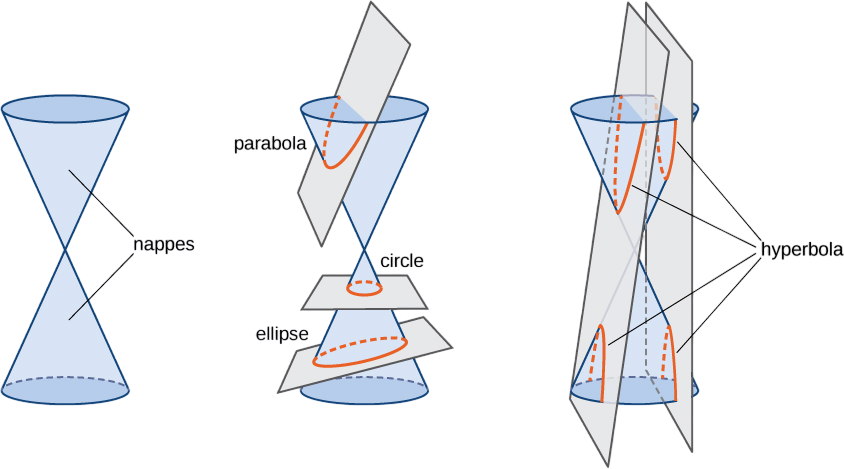
\includegraphics[width=0.8\textwidth]{double-napped cone to 2D shapes.png}
    \caption{Conic sections formed by the intersection of a plane with a double-napped cone.}
\end{figure}
\end{conceptbox}

\section*{Ellipse}
\addcontentsline{toc}{subsection}{Ellipse}
\begin{definitionbox}
An \textbf{ellipse} is the set of all points in a plane such that the sum of their distances to two fixed points (called the \textit{foci}) is constant.
\begin{figure}[H]
    \centering
    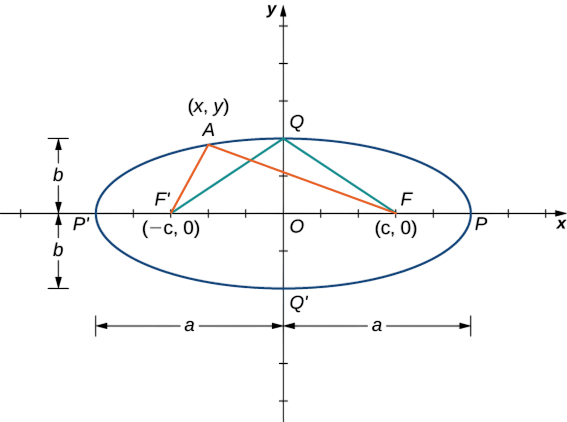
\includegraphics[width=0.65\textwidth]{ellipse.jpg}
    \caption{Diagram of an ellipse.}
\end{figure}

\begin{intuitionbox} 
    Imagine looping a circular string around two fixed points \( F_1 \) and \( F_2 \) on a plane and pulling it taut (fully stretched without slack) with a pencil. As you move the pencil while keeping the string tight, the traced shape forms an ellipse. This method is commonly used for drawing ellipses with nails and string.
    \begin{figure}[H]
        \centering
        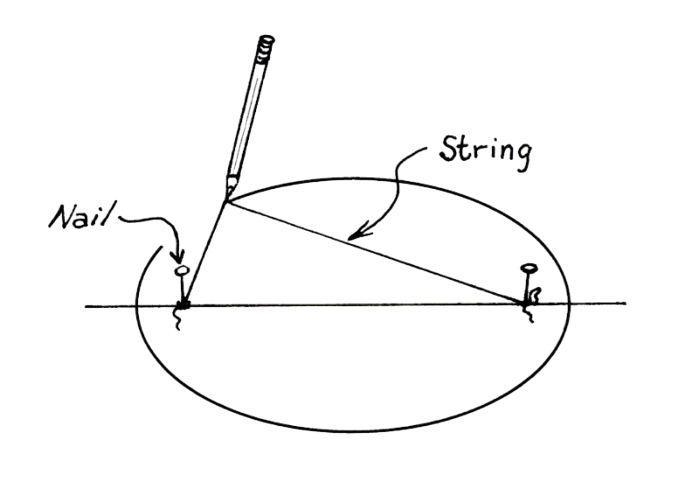
\includegraphics[width=0.4\textwidth]{ellipse_string_example.png}
        \caption{Drawing an ellipse with nails and string.}
    \end{figure}
\end{intuitionbox}
\end{definitionbox}

\subsection*{Standard Forms of an Ellipse}
\addcontentsline{toc}{subsubsection}{Standard Forms of an Ellipse}

\begin{definitionbox}
The equation of an ellipse depends on the orientation of its major axis:

\begin{itemize}
    \item \textbf{Horizontal Major Axis:}  
    \[
    \frac{(x-h)^2}{a^2} + \frac{(y-k)^2}{b^2} = 1
    \]
    where:
    \begin{itemize}
        \item \( (h, k) \) is the center,
        \item \( a > b \) (semi-major axis \( a \), semi-minor axis \( b \)),
        \item \( c^2 = a^2 - b^2 \), where \( c \) is the focal distance.
    \end{itemize}
    
    \item \textbf{Vertical Major Axis:}  
    \[
    \frac{(y-k)^2}{a^2} + \frac{(x-h)^2}{b^2} = 1
    \]
    with the same parameters as above.
\end{itemize}
\begin{remarkbox}
    \textbf{Properties of Ellipses:}
    \begin{itemize}
        \item \textit{Vertices:} Located \( a \) units from the center along the major axis.
        \item \textit{Foci:} Located \( c \) units from the center along the major axis, where \( c^2 = a^2 - b^2 \).
        \item \textit{Eccentricity:} Defined as \( e = \frac{c}{a} \), with \( 0 < e < 1 \).
    \end{itemize}
    \end{remarkbox}
\end{definitionbox}

\subsection*{Verifying an Ellipse}
\addcontentsline{toc}{subsubsection}{Verifying an Ellipse}
\begin{examplebox} 
Show that the equation  
\[
4x^2 + 9y^2 = 36
\]
represents an ellipse and determine its key features.

\begin{solutionbox}
\begin{itemize}
    \item Rewrite the equation in standard form:
    \[
    \frac{x^2}{9} + \frac{y^2}{4} = 1.
    \]
    \item The ellipse is centered at \( (0, 0) \) with \( a = 3 \), \( b = 2 \), and \( c = \sqrt{a^2 - b^2} = \sqrt{5} \).
    \item The foci are \( (\pm \sqrt{5}, 0) \), and the vertices are \( (\pm 3, 0) \).
\end{itemize}
\end{solutionbox}
\end{examplebox}

\section*{Parabola}
\addcontentsline{toc}{subsection}{Parabola}
\begin{definitionbox}
A \textbf{parabola} is the set of all points in a plane equidistant from a fixed point (the \textit{focus}) and a fixed line (the \textit{directrix}).
\begin{figure}[H]
    \centering
    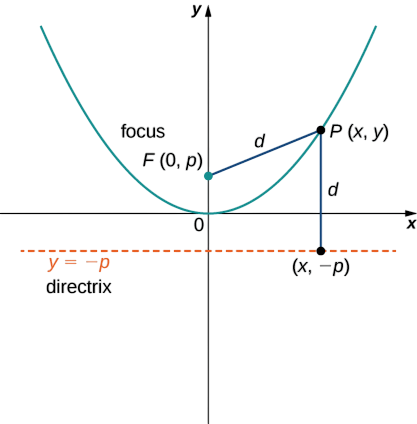
\includegraphics[width=0.45\textwidth]{parabola.jpg}
    \caption{Diagram of a parabola.}
\end{figure}
\begin{intuitionbox}
    A parabola can be thought of as the trajectory of an object under uniform acceleration, such as the path of a ball thrown in the air.
    \begin{figure}[H]
        \centering
        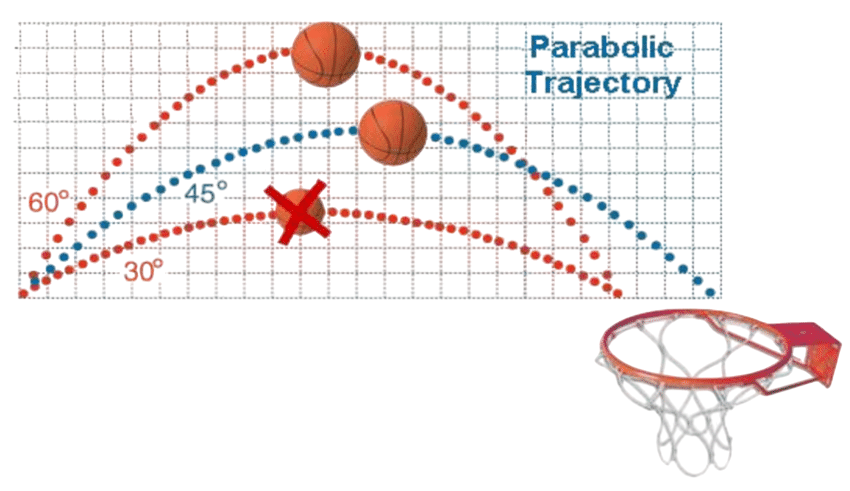
\includegraphics[width=0.65\textwidth]{parabola_ball_example.png}
        \caption{Parabolic trajectory of a ball.}
    \end{figure}
    \end{intuitionbox}
\end{definitionbox}

\subsection*{Standard Forms of a Parabola}
\addcontentsline{toc}{subsubsection}{Standard Forms of a Parabola}

\begin{definitionbox}
The equation of a parabola depends on whether it opens horizontally or vertically:

\begin{itemize}
    \item \textbf{Opens Right or Left (Horizontal Axis):}  
    \[
    (y-k)^2 = 4p(x-h)
    \]
    \begin{itemize}
        \item \( (h, k) \) is the vertex.
        \item \( p \) is the directed distance from the vertex to the focus.
        \item The focus is at \( (h+p, k) \), and the directrix is the vertical line \( x = h - p \).
    \end{itemize}

    \item \textbf{Opens Up or Down (Vertical Axis):}  
    \[
    (x-h)^2 = 4p(y-k)
    \]
    \begin{itemize}
        \item The vertex and \( p \) are the same as above.
        \item The focus is at \( (h, k+p) \), and the directrix is the horizontal line \( y = k - p \).
    \end{itemize}
\end{itemize}
\begin{remarkbox}
    \textbf{Properties of Parabolas:}
    \begin{itemize}
        \item \textit{Focus:} Located \( p \) units from the vertex along the axis of symmetry.
        \item \textit{Directrix:} A line perpendicular to the axis of symmetry at a distance \( p \) from the vertex.
        \item \textit{Axis of Symmetry:} A line that passes through the focus and is perpendicular to the directrix.
    \end{itemize}
    \end{remarkbox}
\end{definitionbox}

\subsection*{Verifying a Parabola}
\addcontentsline{toc}{subsubsection}{Verifying a Parabola}
\begin{examplebox}  
Show that the equation  
\[
y^2 = 12x
\]
represents a parabola and determine its key features.

\begin{solutionbox}
\begin{itemize}
    \item The equation is in the standard form \( y^2 = 4px \), with \( 4p = 12 \), so \( p = 3 \).
    \item The parabola opens to the right, with vertex \( (0, 0) \), focus \( (3, 0) \), and directrix \( x = -3 \).
\end{itemize}
\end{solutionbox}
\end{examplebox}

\section*{Hyperbola}
\addcontentsline{toc}{subsection}{Hyperbola}
\begin{definitionbox}  
A \textbf{hyperbola} is the set of all points in a plane such that the absolute difference of their distances to two fixed points (called the \textit{foci}) is constant.
\begin{figure}[H]
    \centering
    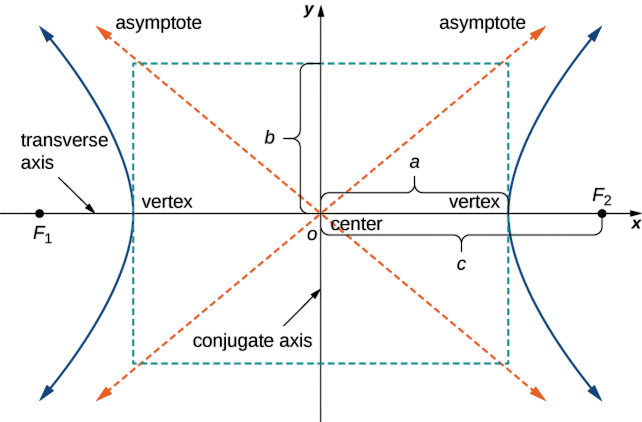
\includegraphics[width=0.75\textwidth]{hyperbola.jpg}
    \caption{Diagram of a hyperbola.}
\end{figure}
\end{definitionbox}

\begin{intuitionbox}
A hyperbola appears in real-world phenomena such as satellite orbits, radio wave propagation, and the paths of comets.
\begin{figure}[H]
    \centering
    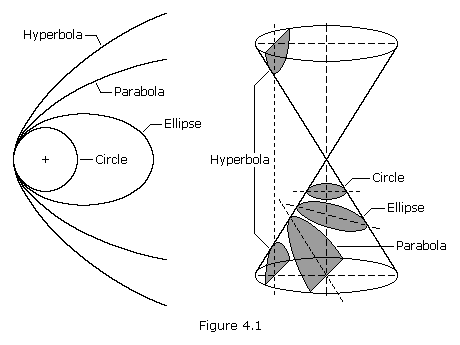
\includegraphics[width=0.5\textwidth]{hyperbola_comparison_to_other_shapes.png}
    \caption{Hyperbolic orbits can have greater eccentricity than parabolic ones.}
\end{figure}
\begin{figure}[H]
    \centering
    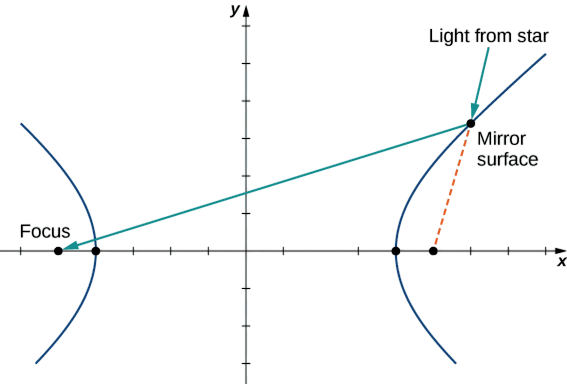
\includegraphics[width=0.75\textwidth]{example_light_hyperbola.jpg}
    \caption{ A hyperbolic mirror used to collect light from distant stars.}
\end{figure}
\end{intuitionbox}

\subsection*{Standard Forms of a Hyperbola}
\addcontentsline{toc}{subsubsection}{Standard Forms of a Hyperbola}
\begin{definitionbox}
    A hyperbola is defined by the difference of distances to two fixed points (foci) being constant. Its standard equation depends on the orientation of its transverse axis:  
    \begin{itemize}
        \item \textbf{Horizontal Transverse Axis:}  
        \[
        \frac{(x-h)^2}{a^2} - \frac{(y-k)^2}{b^2} = 1,
        \]
        where \( (h, k) \) is the center, \( a \) is the distance from the center to each vertex, and \( c^2 = a^2 + b^2 \) defines the distance from the center to each focus.  
        
        \item \textbf{Vertical Transverse Axis:}  
        \[
        \frac{(y-k)^2}{a^2} - \frac{(x-h)^2}{b^2} = 1.
        \]
    \end{itemize}
    \begin{remarkbox}
        \textbf{Properties of Hyperbolas:}
        \begin{itemize}
            \item \textit{Foci:} Located \( c \) units from the center along the transverse axis, where \( c^2 = a^2 + b^2 \).
            \item \textit{Asymptotes:} Lines that the hyperbola approaches but never touches, given by:
            \[
            y = k \pm \frac{b}{a}(x-h) \quad \text{(horizontal)}.
            \]
            \item \textit{Vertices:} Located \( a \) units from the center along the transverse axis.
        \end{itemize}
        \end{remarkbox}
\end{definitionbox}

\subsection*{Verifying a Hyperbola}
\addcontentsline{toc}{subsubsection}{Verifying a Hyperbola}
\begin{examplebox}
Show that the equation  
\[
9x^2 - 16y^2 = 144
\]
represents a hyperbola and determine its key features.

\begin{solutionbox}
\begin{itemize}
    \item Rewrite the equation in standard form:
    \[
    \frac{x^2}{16} - \frac{y^2}{9} = 1.
    \]
    \item The hyperbola is centered at \( (0, 0) \) with \( a = 4 \), \( b = 3 \), and \( c = \sqrt{a^2 + b^2} = 5 \).
    \item The vertices are \( (\pm 4, 0) \), the foci are \( (\pm 5, 0) \), and the asymptotes are \( y = \pm \frac{3}{4}x \).
\end{itemize}
\end{solutionbox}
\end{examplebox}

\section*{Eccentricity and Directrix}
\addcontentsline{toc}{subsection}{Eccentricity and Directrix}

\begin{definitionbox}The \textbf{eccentricity} \( e \) of a conic section is defined as the ratio of the distance from any point on the conic to its focus, divided by the perpendicular distance from that point to the nearest directrix. This value is constant for a given conic and determines its type:
\begin{itemize}
    \item If \( e = 1 \), the conic is a \textbf{parabola}.
    \item If \( e < 1 \), the conic is an \textbf{ellipse}.
    \item If \( e > 1 \), the conic is a \textbf{hyperbola}.
\end{itemize}

\begin{remarkbox}
For a \textbf{circle}, the eccentricity is \( e = 0 \).
\end{remarkbox}

The \textbf{directrix} of a conic section is a fixed line that, together with the focus, helps define the conic. 
\begin{itemize}
    \item \textbf{Parabolas} have one focus and one directrix.
    \item \textbf{Ellipses} and \textbf{hyperbolas} (excluding circles) have two foci and two corresponding directrices.
\end{itemize}
\end{definitionbox}

\begin{illustrationbox}
    \begin{figure}[H]
        \centering
        \begin{minipage}{0.45\textwidth}
            \centering
            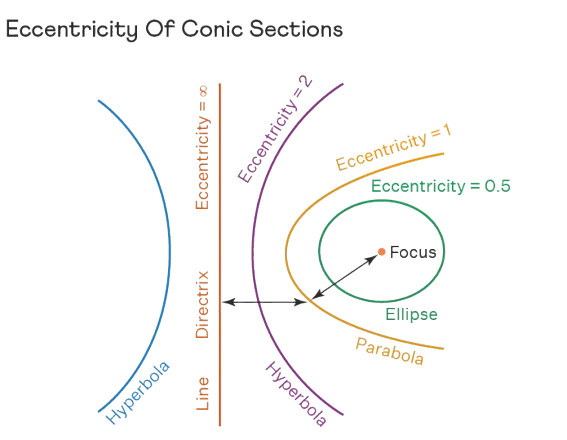
\includegraphics[width=\linewidth]{eccentricity and directrix.png}
            \caption{Eccentricity and directrix of conic sections.}
        \end{minipage}
        \hfill
        \begin{minipage}{0.45\textwidth}
            \centering
            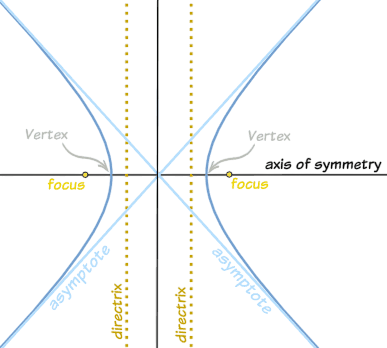
\includegraphics[width=\linewidth]{hyperbola directrix.png}
            \caption{Directrix of a hyperbola.}
        \end{minipage}
        
        \vspace{1em} % Adds vertical space before the next row
        
        \begin{minipage}{0.6\textwidth}
            \centering
            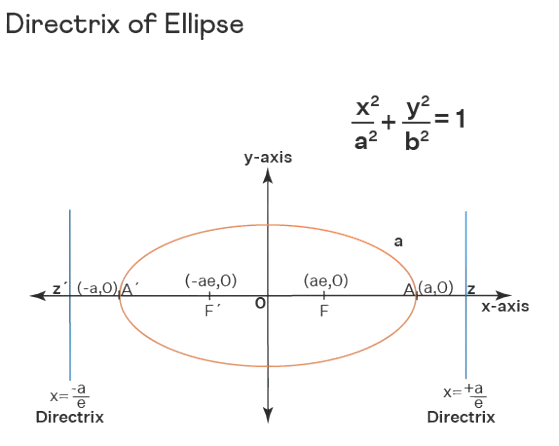
\includegraphics[width=\linewidth]{ellipse directrix.png}
            \caption{Directrix of an ellipse.}
        \end{minipage}
    \end{figure}    
\end{illustrationbox}

\section*{General Equations of Degree Two}
\addcontentsline{toc}{subsection}{General Equations of Degree Two}

\begin{conceptbox}
A general second-degree equation is written as:
\[
Ax^2 + Bxy + Cy^2 + Dx + Ey + F = 0.
\]
The nature of its graph (a conic section) is determined using the \textbf{discriminant}:
\[
\Delta = 4AC - B^2.
\]
\begin{itemize}
    \item If \( \Delta > 0 \), the conic is an \textbf{ellipse}.
    \item If \( \Delta = 0 \), the conic is a \textbf{parabola}.
    \item If \( \Delta < 0 \), the conic is a \textbf{hyperbola}.
\end{itemize}
\begin{remarkbox}
    If \( B \neq 0 \), the coordinate axes are rotated.

    To determine the rotation angle \( \theta \), use:
    \[
    \cot 2\theta = \frac{A - C}{B}.
    \]
\end{remarkbox}
\end{conceptbox}

\section*{Distinguishing Between Conic Sections}
\addcontentsline{toc}{subsection}{Distinguishing Between Conic Sections}

\begin{tipbox}
To classify a conic section, follow these key steps:
\begin{enumerate}
    \item \textbf{Check the discriminant} \( \Delta = 4AC - B^2 \):
    \begin{itemize}
        \item \( \Delta > 0 \) indicates an \textbf{ellipse}.
        \item \( \Delta = 0 \) indicates a \textbf{parabola}.
        \item \( \Delta < 0 \) indicates a \textbf{hyperbola}.
    \end{itemize}
    \item \textbf{Identify the presence of an \( xy \)-term}:
    \begin{itemize}
        \item If \( B \neq 0 \), the axes are rotated.
    \end{itemize}
    \item \textbf{Analyze the equation form}:
    \begin{itemize}
        \item Ellipses and circles have \textbf{both \( x^2 \) and \( y^2 \) terms} with the same sign.
        \item Hyperbolas have \textbf{both \( x^2 \) and \( y^2 \) terms} with opposite signs.
        \item Parabolas have \textbf{only one squared term} (either \( x^2 \) or \( y^2 \), but not both).
    \end{itemize}
\end{enumerate}
\end{tipbox}

\cleardoublepage
\phantomsection
\begin{titlepage}
    \null % Ensures proper alignment with vfill
    \vfill
    \begin{center}
        {\Huge \textbf{Let’s Get Started}} \\[20pt]
        \rule{\textwidth}{0.5mm} \\[15pt]
        {\Large \textit{Time to dive into the lecture notes.}} \\[15pt]
        \rule{\textwidth}{0.5mm} \\[15pt]
        \textbf{Grab your pen or pencil, and let’s break this down step by step.}
    \end{center}
    \vfill
\end{titlepage}

\addcontentsline{toc}{section}{Lecture Content}
\normalsize

\setcounter{page}{1}

\section*{Review from the Previous Lecture}
\addcontentsline{toc}{subsection}{Review from the Previous Lecture}
\begin{remarkbox}
In the previous lecture, we covered important foundational concepts related to polar coordinates and their derivatives. Here’s a brief summary: 

\begin{itemize}
    \item \textbf{Derivative of \( r = f(\theta) \) in Cartesian Coordinates:}
    \large
    \[
        \dfrac{dy}{dx} = \dfrac{\dfrac{dy}{d\theta}}{\dfrac{dx}{d\theta}} = \dfrac{\dfrac{dr}{d\theta}\sin\theta + r\cos\theta}{\dfrac{dr}{d\theta}\cos\theta - r\sin\theta}
    \]
    \normalsize
    This formula helps us compute the slope of the tangent line for polar curves when converted to Cartesian coordinates. 

    \item \textbf{Equation of a Circle:}
    \[
        (x-h)^2 + (y-k)^2 = r^2
    \]
    Here:
    \begin{itemize}
        \item[\labelitemi] \( r \): Radius of the circle
        \item[\labelitemi] \( (h, k) \): Centre of the circle
    \end{itemize}    
\end{itemize}

\begin{notebox}
\textbf{Reminder:} Term Test 1 is scheduled for \textbf{Thursday, January 30th, 2025 (Week 4)}. Make sure to review polar derivatives, transformations, and conic sections!
\end{notebox}
\end{remarkbox}

\section*{Exploring Common Curve Shapes}
\addcontentsline{toc}{subsection}{Exploring Common Curve Shapes}

\subsection*{Parabola}
\addcontentsline{toc}{subsubsection}{Parabola}

\begin{definitionbox}
A \textbf{parabola} is a symmetric curve defined by the quadratic equation:  
\[
    y = ax^2 + bx + c, \quad a \neq 0
\]
To rewrite this equation in vertex form, we complete the square:  
\[
    y = A(x - B)^2 + C
\]

Here:  
\begin{itemize}
    \item \( A \): Determines the direction and "width" of the parabola.  
    \[
        A > 0 \implies \text{The parabola opens upwards.}
    \]  
    \[
        A < 0 \implies \text{The parabola opens downwards.}
    \]
    \item \( (B, C) \): Represents the vertex of the parabola.
    \begin{itemize} 
        \item[\labelitemi] \( B \): Horizontal position of the vertex.  
        \item[\labelitemi] \( C \): Vertical position of the vertex.
    \end{itemize} 
\end{itemize}

\begin{algorithmbox}

    \textbf{Vertex Formula:}  
    To find the vertex when given the standard form \( y = ax^2 + bx + c \), use the formulas:  
    \[
        B = -\frac{b}{2a}, \quad C = f(B)
    \]
    where \( f(B) \) is the value of the quadratic function evaluated at \( x = B \).
\end{algorithmbox}
\end{definitionbox}

\subsection*{Sketching the Region of a Set Defined by a Parabola}
\addcontentsline{toc}{subsubsection}{Sketching the Region of a Set Defined by a Parabola}
\begin{examplebox}
Sketch the region of the set defined by
\[
    R = \{ (x, y) \mid y \geq x^2 + 1 \}.
\]

\begin{remarkbox}
    To sketch the region defined by \( y \geq x^2 + 1 \), we first consider the graph of the parabola \( y = x^2 + 1 \):
    
    \begin{figure}[H]
        \centering
        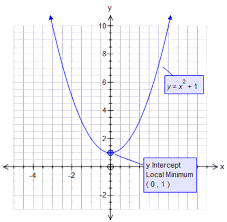
\includegraphics[width=0.4\textwidth]{x^2 + 1.png}
        \caption{Graph of \( y = x^2 + 1 \).}
        \label{fig:parabola_graph}
    \end{figure}
    
    Next, let’s test some sample points to determine whether they lie in the region \( y \geq x^2 + 1 \):  
    
    \begin{itemize}
        \item For the point \( (-2, 0) \):  
        \[
        y \geq x^2 + 1 \implies 0 \geq (-2)^2 + 1 \implies 0 \geq 5,
        \]
        which is \textbf{false}. Therefore, \( (-2, 0) \) is not in the region.
        
        \item For the point \( (0, 2) \):  
        \[
        y \geq x^2 + 1 \implies 2 \geq 0^2 + 1 \implies 2 \geq 1,
        \]
        which is \textbf{true}. Therefore, \( (0, 2) \) is in the region.
    \end{itemize}
\end{remarkbox}

\textit{...cont'd...}
\end{examplebox}

\begin{examplebox}
\textit{...cont'd...}
\begin{solutionbox}
    The region defined by \( y \geq x^2 + 1 \) is shown below:

    \begin{blankbox}
        \begin{figure}[H]
            \centering
            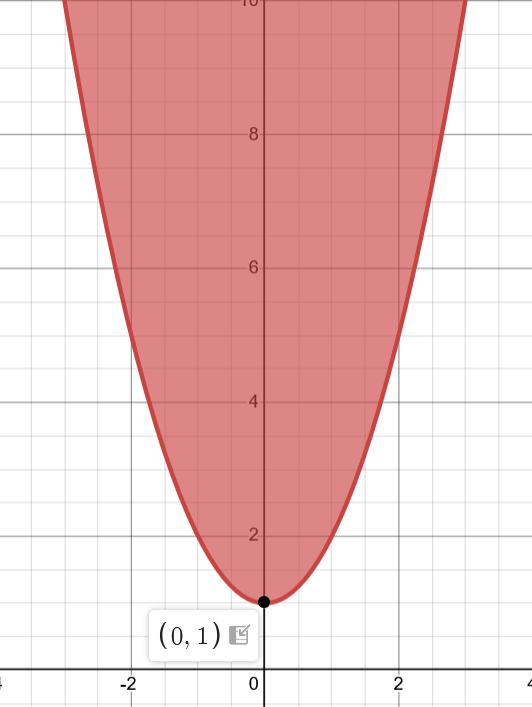
\includegraphics[width=0.4\textwidth]{y = x^2 + 1 shaded.png}
            \caption{Shaded region satisfying \( y \geq x^2 + 1 \).}
            \label{fig:region}
        \end{figure}
    \end{blankbox}
    
    \textbf{How to Determine the Region:}
    \begin{conceptbox}
    To determine the region for \( y \geq x^2 + 1 \):
    \begin{itemize}
        \item The parabola \( y = x^2 + 1 \) acts as a boundary. The inequality \( y \geq x^2 + 1 \) indicates that the region lies above or on this parabola.
        \item The graph of \( y = x^2 + 1 \) opens upwards, so the region \( R \) is the area above this curve, including the curve itself.
        \item The boundary curve \( y = x^2 + 1 \) is part of the region because the inequality includes equality (\( \geq \)).
    \end{itemize}
    \end{conceptbox}
\end{solutionbox}    
\end{examplebox}

\subsection*{Ellipse}
\addcontentsline{toc}{subsubsection}{Ellipse}
\begin{definitionbox}
The equation of an ellipse is defined by
\[
    \dfrac{(x - h)^2}{a^2} + \dfrac{(y - k)^2}{b^2} = 1 \text{.}
\]
\begin{remarkbox}
Recall the equation of the circle, which is based on the equation of the ellipse when \( a = b = 1 \):
\[
    \text{Circle:} \quad (x - h)^2 + (y - k)^2 = r^2 \text{,}
\]
where \( (h, k) \) is the centre, \( a \) represents the \( x \)-axis radius, and \( b \) represents the \( y \)-axis radius.
\end{remarkbox}
\end{definitionbox}

\subsection*{Sketching the Region of a Set Defined by an Ellipse}
\addcontentsline{toc}{subsubsection}{Sketching the Region of a Set Defined by an Ellipse}

\begin{examplebox}
Sketch the region of the set defined by
\[
    A = \{ (x, y) \mid x^2 + 4y^2 > 4 \}.
\]

\begin{remarkbox}
    To sketch the region defined by \( x^2 + 4y^2 > 4 \), we first consider the graph of the ellipse \( x^2 + 4y^2 = 4 \):

    \begin{figure}[H]
        \centering
        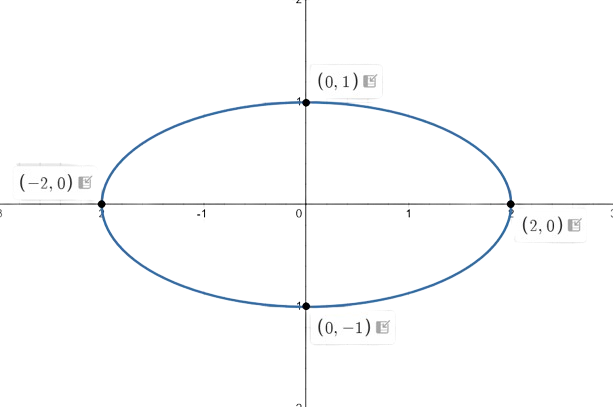
\includegraphics[width=0.65\textwidth]{graph of x^2 + 4y^2 = 4.png}
        \caption{Graph of \( x^2 + 4y^2 = 4 \).}
        \label{fig:ellipse_graph}
    \end{figure}

    Next, let’s test some sample points to determine whether they lie in the region \( x^2 + 4y^2 > 4 \):

    \begin{itemize}
        \item For the point \( (0, 0) \):
        \[
        x^2 + 4y^2 > 4 \implies 0^2 + 4(0)^2 > 4 \implies 0 > 4,
        \]
        which is \textbf{false}. Therefore, \( (0, 0) \) is not in the region.

        \item For the point \( (3, 0) \):
        \[
        x^2 + 4y^2 > 4 \implies 3^2 + 4(0)^2 > 4 \implies 9 > 4,
        \]
        which is \textbf{true}. Therefore, \( (3, 0) \) is in the region.
    \end{itemize}
\end{remarkbox}

\textit{...cont'd...}
\end{examplebox}

\begin{examplebox}
\textit{...cont'd...}
\begin{solutionbox}
    The region defined by \( x^2 + 4y^2 > 4 \) is shown below:

    \begin{blankbox}
        \begin{figure}[H]
            \centering
            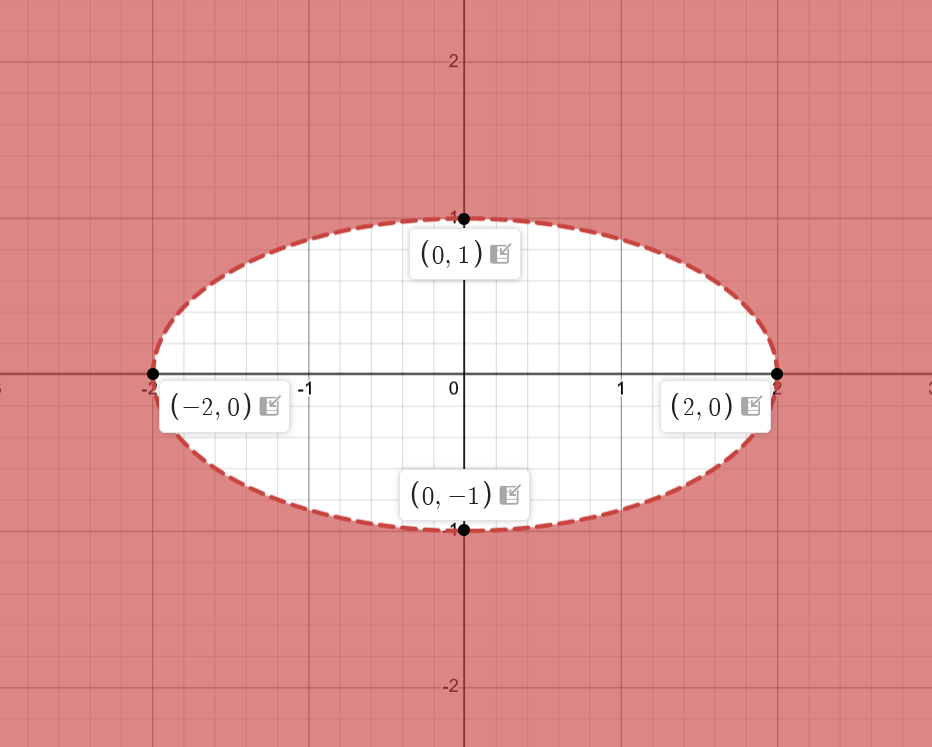
\includegraphics[width=0.4\textwidth]{x^2 + 4y^2 gt 4 region.png}
            \caption{Shaded region satisfying \( x^2 + 4y^2 > 4 \).}
            \label{fig:ellipse_region}
        \end{figure}
    \end{blankbox}

    \textbf{How to Determine the Region:}
    \begin{conceptbox}
    To determine the region for \( x^2 + 4y^2 > 4 \):
    \begin{itemize}
        \item The ellipse \( x^2 + 4y^2 = 4 \) acts as a boundary. The inequality \( x^2 + 4y^2 > 4 \) indicates that the region lies outside this ellipse.
        \item The equation can be rewritten as \( \frac{x^2}{4} + \frac{y^2}{1} = 1 \), showing that it is an ellipse centered at \( (0,0) \) with a semi-major axis of 2 (along \( x \)-axis) and a semi-minor axis of 1 (along \( y \)-axis).
        \item The boundary curve \( x^2 + 4y^2 = 4 \) is \textbf{not} part of the region because the inequality is strict (\( > \)).
        \item A dashed boundary is used in the sketch to indicate that the ellipse itself is not included in the region.
    \end{itemize}
    \end{conceptbox}
\end{solutionbox}    
\end{examplebox}

\section*{Introducing the Hyperbola}
\begin{definitionbox}
The equation of a hyperbola is defined by
\[
    \dfrac{x^2}{a^2} - \dfrac{y^2}{b^2} = 1
\]
\begin{illustrationbox}
    \textbf{self-note: add the image of the corresponding illustration here (see the lecture note)}
    \begin{figure}[H]
        \centering
        
\includegraphics[width=0.35\textwidth]{sample_image.jpg}
        \caption{Sample image illustrating the concept.}
        \label{fig:sample_image}
    \end{figure}
\end{illustrationbox}
\[
    \dfrac{y^2}{b^2} - \dfrac{x^2}{a^2} = 1
\]
\begin{illustrationbox}
    \textbf{self-note: add the image of the corresponding illustration here (see the lecture note)}
    \begin{figure}[H]
        \centering
        
\includegraphics[width=0.35\textwidth]{sample_image.jpg}
        \caption{Sample image illustrating the concept.}
        \label{fig:sample_image}
    \end{figure}
\end{illustrationbox}
\end{definitionbox}

\section*{Welcome to Linear Algebra...}
\subsection*{well... not really!}

\section*{Section 2.1/2.2: Welcome to 3D Space!}
\begin{remarkbox}
Recall that the cartesian coordinate system considers the 2-dimensional realm: a system in \( \mathbb{R}^2 \).
\begin{illustrationbox}
    \textbf{self-note: add the cartesian plane — the typical one in 2D}
    \begin{figure}[H]
        \centering
        
\includegraphics[width=0.35\textwidth]{sample_image.jpg}
        \caption{Sample image illustrating the concept.}
        \label{fig:sample_image}
    \end{figure}
\end{illustrationbox}
Now, check out the cartesian coordinate system being introduced in MAT232, considering the 3-dimensional realm; \( \mathbb{R}^3 \):
\begin{illustrationbox}
    \textbf{self-note: add the illustration for the 3D cartesian plane, the z-axis in addition to the x- and \( y \)-axis}.
    \begin{figure}[H]
        \centering
        
\includegraphics[width=0.35\textwidth]{sample_image.jpg}
        \caption{Sample image illustrating the concept.}
        \label{fig:sample_image}
    \end{figure}
\end{illustrationbox}
\end{remarkbox}

\begin{notebox}
\underline{In 2D:} \\
Notice that \( \mathbb{R}^2 = \mathbb{R} \times \mathbb{R} \), where the first \( \mathbb{R} \) represents the \( x \)-values and the second \( \mathbb{R} \) represents the \( y \)-values.
\\
\underline{Now, in 3D:} \\
Notice that \( \mathbb{R}^3 = \mathbb{R} \times \mathbb{R} \times \mathbb{R} \).
\begin{itemize}
    \item The first \( \mathbb{R} \) represents the \( x \)-values;
    \item The second \( \mathbb{R} \) represents the \( y \)-values;
    \item The third \( \mathbb{R} \) represents the \( z \)-values.
\end{itemize}
\end{notebox}

\section*{Example of Plotting in a 3D Cartesian Plane}
\begin{examplebox}
Plot the points \( (-1, 2, -3) \) and \( (2, -4, 2) \).
\begin{illustrationbox}
    \textbf{self-note: add the illustration here!!}
    \begin{figure}[H]
        \centering
        
\includegraphics[width=0.35\textwidth]{sample_image.jpg}
        \caption{Sample image illustrating the concept.}
        \label{fig:sample_image}
    \end{figure}
\end{illustrationbox}
\textit{Follow the line segments denoted in \textbf{purple} for an interpretation guide of how the three components contribute to the final point destination, for \( (-1, 2, -3) \).} \\
\textit{Follow the line segments denoted in \textbf{green} for an interpretation guide of how the three components contribute to the final point destination, for \( (2, -4, 2) \).} \\
\end{examplebox}

\section*{Interpreting Planes}
\begin{conceptbox}
Notice that in a 2D world, there is no notion of height when considering the \( x, y \)-plane. In a 3D world, \( z = 0 \). \\
\\
Now, have a look at the basic planes for a 3D cartesian graph: \\
\\
\underline{The \( xy \) plane:}
\[
    x = 0 \quad\quad\quad (x, y, 0)
\]
\begin{figure}[H]
    \centering
    
\includegraphics[width=0.35\textwidth]{sample_image.jpg}
    \caption{Sample image illustrating the concept.}
    \label{fig:sample_image}
\end{figure}
\underline{The \( yz \) plane:}
\[
    x = 0 \quad\quad\quad (0, y, z)
\]
\begin{figure}[H]
    \centering
    
\includegraphics[width=0.35\textwidth]{sample_image.jpg}
    \caption{Sample image illustrating the concept.}
    \label{fig:sample_image}
\end{figure}
\underline{The \( xz \) plane:}
\[
    x = 0 \quad\quad\quad (x, 0, z)
\]
\begin{figure}[H]
    \centering
    
\includegraphics[width=0.35\textwidth]{sample_image.jpg}
    \caption{Sample image illustrating the concept.}
    \label{fig:sample_image}
\end{figure}
\end{conceptbox}

\section*{Let's Try Going from 2D to 3D}
\begin{examplebox}
Consider the graph defined by \( y = 2 \) on a 2D cartesian graph:
\begin{figure}[H]
    \centering
    
\includegraphics[width=0.35\textwidth]{sample_image.jpg}
    \caption{Sample image illustrating the concept.}
    \label{fig:sample_image}
\end{figure}
Here's how that would look like in a 3D cartesian space:
\begin{figure}[H]
    \centering
    
\includegraphics[width=0.35\textwidth]{sample_image.jpg}
    \caption{Sample image illustrating the concept.}
    \label{fig:sample_image}
\end{figure}
\end{examplebox}

\begin{examplebox}
Consider the graph of a circle defined by
\[
    x^2 + y^2 = 4 \text{.}
\]
\begin{figure}[H]
    \centering
    
\includegraphics[width=0.35\textwidth]{sample_image.jpg}
    \caption{Sample image illustrating the concept.}
    \label{fig:sample_image}
\end{figure}
If this circle is brought to the 3D world, stretched along the \( z \)-axis, for any values of \( z \), then a cylinder is created (the cirle is the cross-section shape).
\begin{figure}[H]
    \centering
    
\includegraphics[width=0.35\textwidth]{sample_image.jpg}
    \caption{Sample image illustrating the concept.}
    \label{fig:sample_image}
\end{figure}
\end{examplebox}

\subsection*{Next Lecture: We Discuss Vectors!}

\section*{Lecture Title}
\begin{notebox}
This template is designed for MAT232 lecture notes. Replace this content with your specific lecture details.
\end{notebox}

\section*{Key Concepts}
\begin{definitionbox}
A \textbf{parametric equation} is a set of equations that express the coordinates of the points of a curve as functions of a variable, called a parameter.
\end{definitionbox}

\section*{Examples}
\begin{examplebox}
\textbf{Example 1:} Consider the parametric equations:
\[ x = t, \quad y = t^2, \quad t \in \mathbb{R}. \]
\begin{itemize}
    \item At $t = 0$, $(x, y) = (0, 0)$.
    \item At $t = 1$, $(x, y) = (1, 1)$.
\end{itemize}
This describes a parabola.

\begin{figure}[H]
    \centering
    
\includegraphics[width=0.35\textwidth]{sample_image.jpg}
    \caption{Sample image illustrating the concept.}
    \label{fig:sample_image}
\end{figure}

\end{examplebox}

\section*{Theorems and Proofs}
\begin{theorembox}
\textbf{Theorem:} If $x(t)$ and $y(t)$ are differentiable functions, the slope of the curve is given by:
\[ \frac{dy}{dx} = \frac{\frac{dy}{dt}}{\frac{dx}{dt}}, \quad \text{provided } \frac{dx}{dt} \neq 0. \]

\begin{figure}[H]
    \centering
    
\includegraphics[width=0.35\textwidth]{sample_image1.jpg}
    \caption{Graphical representation of the theorem.}
    \label{fig:sample_image1}
\end{figure}

\end{theorembox}

\section*{Additional Notes}
\begin{notebox}
Always check the domain of the parameter $t$ when solving problems involving parametric equations.
\end{notebox}

\end{document}
